\documentclass{article}
\usepackage{graphicx}

\title{The Euclidean Algorithm}
\author{William Y. Feng}

\begin{document}

\maketitle
The \textit{greatest common divisor} (gcd) of two integers $a$ and $b$, written $\gcd(a, b)$, is defined as the greatest positive integer that divides both $a$ and $b$.

For example, the gcd of 54 and 30 is 6, because 6 divides both 54 and 30, while no larger integer has this property.

The greatest common divisor operation is a familiar operation to number theorists. In a theoretical setting, mathematicians rarely have to find the greatest common divisor of two cold hard numbers. But we're not going to talk about vague, general things here! We're going to find out how to actually compute the gcd of any two given numbers.

\textbf{A special property of the gcd:} We know that 6 divides both 54 and 30. Notice how 6 also divides their difference: $54 - 30 = 24$. 6 also divides their \textit{sum}, $54 + 30 = 84$. This fact holds in general: if an integer $n$ is a divisor of both $a$ and $b$, then it divides $a - b$ and $a + b$ as well.

Coincidentally, this holds for the gcd too:

\textbf{Big Claim.} If $n$ is the greatest common divisor of $a$ and $b$, then $n$ is also the greatest common divisor of $b$ and $a - b$.

To see why this is true, assume otherwise; perhaps there exists a larger number $d$ that divides both $b$ and $a - b$. But then, according to our facts above, $d$ would divide $b + (a - b) = a$ too, contradicting our assumption that 6 was the \textit{greatest} common divisor of $a$ and $b$.

Now, let's put this to use and find the greatest common divisor of 49 and 63. Maybe it's already obvious to you what the answer is, but play along! Again, this is the largest positive integer that is a divisor of both 49 and 63. Let this number be $d$.

One thing we certainly \textit{don't} want to do is test a bunch of numbers and determine the largest one that divides both 49 and 63. What we can do instead is apply the Big Claim: we know that $d$ should also be the greatest common divisor of 49 and the \textit{difference} between 49 and 63,
$$63 - 49 = 14.$$
So now we have reduced the problem to finding the greatest common divisor of 49 and \textit{14}. In other words, we
$$\gcd(49, 63) = \gcd(49, 14).$$
This seems good; we've essentially gotten rid of a big number, 63, and replaced it with a smaller number, 14.

To find $\gcd(49, 14)$, we can apply the Big Claim again! This time, we subtract 14 from 49 to get 35:
$$\gcd(49, 14) = \gcd(35, 14).$$
We can do it again, subtracting 14 from 35:
$$\gcd(35, 14) = \gcd(21, 14)$$
and again:
$$\gcd(21, 14) = \gcd(7, 14).$$
Now we subtract 7 from 14 to get
$$\gcd(7, 14) = \gcd(7, 7),$$
and then one last time to get
$$\gcd(7, 7) = \gcd(7, 0).$$
The greatest common divisor of zero and another number is always the other number, because everything divides zero. Thus, $\gcd(7, 0) = 7$. Condensing all our steps, we see that we went from
$$\gcd(49, 63) = \gcd(7, 0) = 7,$$
solely by applying the Big Claim. And we see that throughout all our reductions, 7 remained the greatest common divisor of both number.

\begin{center}

\includegraphics[scale=0.7]{images/euclidean.png}
\end{center}

This is the process behind the \textbf{Euclidean Algorithm}: To find the gcd of $a$ and $b$, we can subtract the smaller number from the larger number to reduce the overall size of the two numbers. From there, we rinse and repeat until we get down to sufficiently small numbers to determine the answer directly.

\textbf{A small problem:} Suppose we're trying to find the gcd of 15174 and 702. The answer isn't immediately obvious, so we try the subtraction trick by turning 15174 into $15174 - 702 = 14472$. We get
$$\gcd(702, 15174) = \gcd(702, 14472).$$
Still not obvious what the answer is, so let's try again, this time replacing $14472$ with $14472 - 702 = 13770$:
$$\gcd(702, 14472) = \gcd(702, 13370).$$
If we keep doing this---subtracting 702 from the second number---we'll eventually get down to
\begin{align*}
\gcd(702, 1134) & = \gcd(702, 1134 - 702) \\
    & = \gcd(702, 432)
\end{align*}

This livens things up a bit and now we can instead subtract 432 from 702. But was there a better way to get here? Let's look at the original query:
$$\gcd(702, 15174)$$
Evidently we'll be subtracting 702 from the second number for a while. Instead of doing all these subtractions, we can just do them all at once and \textit{take the remainder} with 15174 by 702. Perhaps this is best illustrated by calculating the quotient and remainder:
$$15174 = 21(702) + 432.$$
Essentially, we'll subtract 702 from the first number a whopping \textit{21 times} before the first number becomes 432 and we can start subtracting from 702 instead. In this case, 432 is the \textit{remainder} when 15174 is divided by 702.

In general, if we want o find $\gcd(a, b)$ and $b$ is smaller than $a$, then we know that this gcd equals $\gcd(a\,\%\,b, b)$, where $a\,\%\,b$ denotes the remainder when $a$ is divided by $b$. If we apply \textit{this} until we get one of the arguments down to zero, we get \textit{54} as the gcd of 702 and 15174.

\textbf{Summary:} Putting it all together, we get the following algorithm:
\begin{enumerate}
\item Take two numbers, $a$ and $b$. Possibly reorder them so that $a < b$.
\item Subtract the smaller number from the larger one as much as possible (using the remainder operation to speed things up).
\item Once one of the numbers becomes 0, the other number is the gcd.
\end{enumerate}
The Euclidean Algorithm has many applications in algorithmic number theory—one of them involves extending the algorithm to find \textit{modular inverses}, a critical component in cryptographic protocols such as the \textit{Diffie-Hellman key exchange} and the \textit{RSA} encryption scheme.
\begin{center}
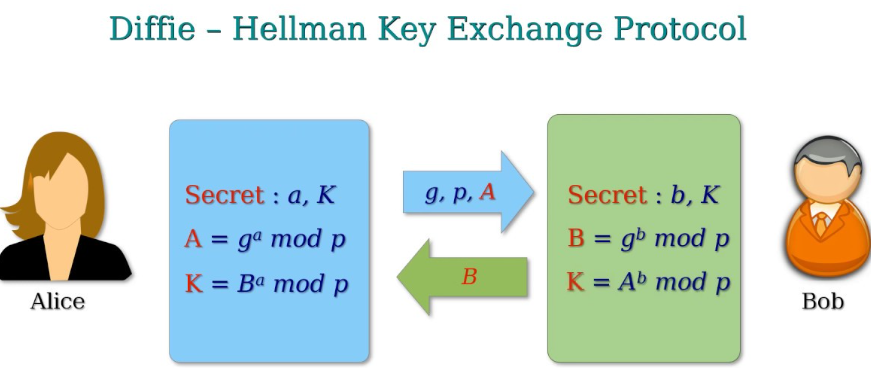
\includegraphics[scale=0.4]{images/diffie_hellman.png}
\end{center}
\end{document}